\chapter{Logistic Regression}


\section{Representation}
Logistic regression can be binomial or multinomial. The \textbf{binomial logistic regression} model has the following form
\begin{equation}
p(y|\vec{x},\vec{w})=\mathrm{Ber}(y|\mathrm{sigm}(\vec{w}^T\vec{x}))
\end{equation}
where $\vec{w}$ and $\vec{x}$ are extended vectors, i.e., $\vec{w}=(b, w_1, w_2,\cdots, w_D)$, $\vec{x}=(1, x_1, x_2,\cdots, x_D)$.


\section{Optimization}
\label{sec:binomial-LR-Optimization}

\subsection{MLE}
\begin{align}
\ell(\vec{w}) &= \log\left\{\prod\limits_{i=1}^N{\left[\pi(\vec{x}_i)\right]^{y_i}\left[1-\pi(\vec{x}_i)\right]^{1-y_i}}\right\} \nonumber \\
              & \quad \text{, where } \pi(\vec{x}) \triangleq P(y=1|\vec{x},\vec{w}) \nonumber \\
           &= \sum\limits_{i=1}^N\left[y_i\log\pi(\vec{x}_i)+(1-y_i)\log(1-\pi(\vec{x}_i))\right] \label{eqn:cross-entropy-error} \nonumber \\
		   &= \sum\limits_{i=1}^N\left[y_i\log\dfrac{\pi(\vec{x}_i)}{1-\pi(\vec{x}_i)}+\log(1-\pi(\vec{x}_i))\right] \nonumber \\
		   &= \sum\limits_{i=1}^N\left[y_i(\vec{w}\cdot\vec{x}_i)-\log(1+\exp(\vec{w}\cdot\vec{x}_i))\right] \nonumber \\
J(\vec{w}) & \triangleq \mathrm{NLL}(\vec{w})= -\ell(\vec{w}) \nonumber \\
           & = -\sum\limits_{i=1}^N\left[y_i(\vec{w}\cdot\vec{x}_i)-\log(1+\exp(\vec{w}\cdot\vec{x}_i))\right] 
\end{align}

Equation \ref{eqn:cross-entropy-error} is also called the \textbf{cross-entropy} error function (see Equation \ref{eqn:cross-entropy}).

Unlike linear regression, we can no longer write down the MLE in closed form. Instead, we need to use an optimization algorithm to compute it, see Appendix \ref{chap:Optimization-methods}. For this, we need to derive the gradient and Hessian.

In the case of logistic regression, one can show that the gradient and Hessian of this are given by the following
\begin{align}
\vec{g}(\vec{w}) &= \dfrac{\mathrm{d} J}{\mathrm{d} \vec{w}} = \sum\limits_{i=1}^N \left[\pi(\vec{x}_i) - y_i \right]\vec{x}_i = \vec{X}(\vec{\pi}-\vec{y})\\
\vec{H}(\vec{w}) &= \dfrac{\mathrm{d} \vec{g}^T}{\mathrm{d} \vec{w}}= \dfrac{\mathrm{d}}{\mathrm{d} \vec{w}} (\vec{\pi}-\vec{y})^T\vec{X}^T \nonumber \\
        &= \dfrac{\mathrm{d}}{\mathrm{d} \vec{w}} \vec{\pi}^T\vec{X}^T \nonumber \\
		&= (\pi(\vec{x}_i)(1-\pi(\vec{x}_i))\vec{x}_i, \cdots,)\vec{X}^T \nonumber \\
		&= \vec{X}\vec{S}\vec{X}^T, \quad \vec{S} \triangleq \mathrm{diag}(\pi(\vec{x}_i)(1-\pi(\vec{x}_i))\vec{x}_i)
\end{align}


\subsubsection{Iteratively reweighted least squares (IRLS)}
\label{sec:IRLS}
TODO


\subsection{MAP}
Just as we prefer ridge regression to linear regression, so we should prefer MAP estimation for logistic regression to computing the MLE. 
$\ell_2$ regularization

we can use $\ell_2$ regularization, just as we did with ridge regression. We note that the new objective, gradient and Hessian have the following forms:
\begin{align}
J'(\vec{w}) & \triangleq \mathrm{NLL}(\vec{w})+\lambda \vec{w}^T\vec{w} \\
\vec{g}'(\vec{w}) &= \vec{g}(\vec{w})+\lambda\vec{w} \\
\vec{H}'(\vec{w}) &= \vec{H}(\vec{w})+\lambda\vec{I}
\end{align}

It is a simple matter to pass these modified equations into any gradient-based optimizer.


\section{Multinomial logistic regression}


\subsection{Representation}
\textbf{Multinomial logistic regression} model is also called a \textbf{maximum entropy classifier}, which has the following form
\begin{align}
p(y=c|\vec{x},\vec{W}) & =\dfrac{\exp(\vec{w}_c^T\vec{x})}{\sum_{c=1}^C \exp(\vec{w}_c^T\vec{x})}
\end{align}


\subsection{MLE}
Let $\vec{y}_i=(\mathbb{I}(y_i=1),\mathbb{I}(y_i=1),\cdots, \mathbb{I}(y_i=C))$, $\vec{\mu}_i=(p(y=1|\vec{x}_i,\vec{W}),p(y=2|\vec{x}_i,\vec{W}),\cdots, p(y=C|\vec{x}_i,\vec{W}))$, then the log-likelihood function can be written as
\begin{align}
\ell(\vec{W}) & =\log\prod\limits_{i=1}^N\prod\limits_{c=1}^C \mu_{ic}^{y_{ic}}=\sum\limits_{i=1}^N\sum\limits_{c=1}^C y_{ic}\log \mu_{ic} \\
     & = \sum\limits_{i=1}^N\left[\left(\sum\limits_{c=1}^C y_{ic}\vec{w}_c^T\vec{x}_i\right)-\log\left(\sum\limits_{c=1}^C \exp(\vec{w}_c^T\vec{x}_i)\right)\right]
\end{align}

Define the objective function as NLL
\begin{equation}
J(\vec{W})=\mathrm{NLL}(\vec{W})=-\ell(\vec{W})
\end{equation}

Define $\vec{A} \otimes \vec{B}$ be the \textbf{kronecker product} of matrices $\vec{A}$ and $\vec{B}$.If $\vec{A}$ is an $m \times n$ matrix and $\vec{B}$ is a $p \times q$ matrix, then $\vec{A} \otimes \vec{B}$ is the $mp \times nq$ block matrix
\begin{equation}
\vec{A} \otimes \vec{B} \triangle \left(\begin{array}{ccc}
a_{11}\vec{B} & \cdots & a_{1n}\vec{B} \\
\vdots & \vdots & \vdots \\
a_{m1}\vec{B} & \cdots & a_{mn}\vec{B}
\end{array}\right)
\end{equation}

The gradient and Hessian are given by
\begin{align}
\vec{g}(\vec{W}) & =\sum\limits_{i=1}^N (\vec{\mu}-\vec{y}_i) \otimes \vec{x}_i \\
\vec{H}(\vec{W}) & =\sum\limits_{i=1}^N (\mathrm{diag}(\vec{\mu}_i)-\vec{\mu}_i\vec{\mu}_i^T) \otimes (\vec{x}_i\vec{x}_i^T)
\end{align}
where $\vec{y}_i=(\mathbb{I}(y_i=1),\mathbb{I}(y_i=1),\cdots, \mathbb{I}(y_i=C-1))$ and $\vec{\mu}_i=(p(y=1|\vec{x}_i,\vec{W}),p(y=2|\vec{x}_i,\vec{W}),\cdots, p(y=C-1|\vec{x}_i,\vec{W}))$ are column vectors of length $C-1$.

Pass them to any gradient-based optimizer.


\subsection{MAP}
The new objective
\begin{align}
J'(\vec{W}) & =\mathrm{NLL}(\vec{w})-\log{p(\vec{W})} \\
            & \quad \text{, where } p(\vec{W}) \triangleq \prod\limits_{c=1}^C \mathcal{N}(\vec{w}_c|\vec{0},\vec{V}_0) \nonumber \\
   & = J(\vec{W})+\dfrac{1}{2}\sum\limits_{c=1}^C \vec{w}_c\vec{V}_0^{-1}\vec{w}_c \\
\end{align}

Its gradient and Hessian are given by
\begin{align}
\vec{g}'(\vec{w}) & =\vec{g}(\vec{W})+\vec{V}_0^{-1}\left(\sum\limits_{c=1}^C \vec{w}_c\right) \\
\vec{H}'(\vec{w}) & =\vec{H}(\vec{w})+\vec{I_C} \otimes \vec{V}_0^{-1}
\end{align}

This can be passed to any gradient-based optimizer to find the MAP estimate. Note, however, that the Hessian has size $((CD)×(CD))$, which is $C$ times more row and columns than in the binary case, so limited memory BFGS is more appropriate than Newton’s method.


\section{Bayesian logistic regression}
It is natural to want to compute the full posterior over the parameters, $p(\vec{w}|\mathcal{D})$, for logistic regression models. This can be useful for any situation where we want to associate confidence intervals with our predictions (e.g., this is necessary when solving contextual bandit problems, discussed in Section TODO).

Unfortunately, unlike the linear regression case, this cannot be done exactly, since there is no convenient conjugate prior for logistic regression. We discuss one simple approximation below; some other approaches include MCMC (Section TODO), variational inference (Section TODO), expectation propagation (Kuss and Rasmussen 2005), etc. For notational simplicity, we stick to binary logistic regression.


\subsection{Laplace approximation}


\subsection{Derivation of the BIC}


\subsection{Gaussian approximation for logistic regression}
\label{sec:Gaussian-approximation-for-logistic-regression}


\subsection{Approximating the posterior predictive}


\subsection{Residual analysis (outlier detection) *}


\section{Online learning and stochastic optimization}
Traditionally machine learning is performed \textbf{offline}, however, if we have \textbf{streaming data}, we need to perform \textbf{online learning}, so we can update our estimates as each new data point arrives rather than waiting until “the end” (which may never occur). And even if we have a batch of data, we might want to treat it like a stream if it is too large to hold in main memory. Below we discuss learning methods for this kind of scenario.

TODO


\subsection{The perceptron algorithm}

\subsubsection{Representation}
\begin{equation}
\mathcal{H}:y=f(\vec{x})=\text{sign}(\vec{w}^T\vec{x}+b)
\end{equation}
where $\text{sign}(x)=\begin{cases}+1, & x \geq 0\\-1, & x<0\\\end{cases}$, see Fig. \ref{fig:perceptron}\footnote{\url{https://en.wikipedia.org/wiki/Perceptron}}.

\begin{figure}[hbtp]
\centering
    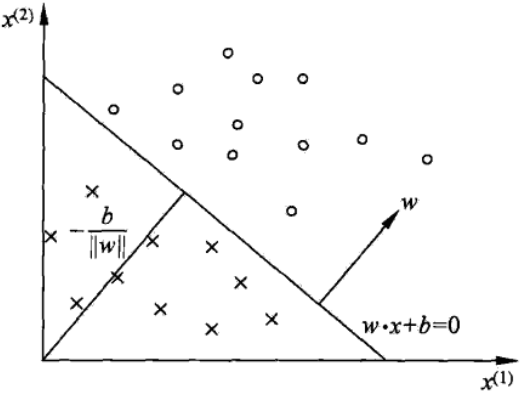
\includegraphics[scale=.50]{perceptron.png}
\caption{Perceptron}
\label{fig:perceptron} 
\end{figure}


\subsubsection{Evaluation}
\begin{eqnarray}
L(\vec{w},b)&=&-y_i(\vec{w}^T\vec{x}_i+b)\\
R_{emp}(f)&=&-\sum\limits_i y_i(\vec{w}^T\vec{x}_i+b)\\
\end{eqnarray}


\subsubsection{Optimization}
\textbf{Primal form}
\begin{algorithm}[htbp]
\caption{Perceptron learning algorithm, primal form, using SGD}
  
    $\vec{w} \leftarrow 0;\; b \leftarrow 0;\; k \leftarrow 0$\;
    \While{no mistakes made within the for loop}{
        \For{$i\leftarrow 1$ \KwTo $N$}{
			\If{$y_i(\vec{w} \cdot \vec{x}_i+b) \leq 0$}{
				$\vec{w} \leftarrow \vec{w}+\eta y_i \vec{x}_i$\;
				$b \leftarrow b+\eta y_i$\;
				$k \leftarrow k+1$\;
			}
		}
    }
\end{algorithm}

\textbf{Convergency}
\begin{theorem}
(\textbf{Novikoff}) If traning data set $\mathcal{D}$ is linearly separable, then
\begin{enumerate}
\item There exists a hyperplane denoted as $\widehat{\vec{w}}_{opt} \cdot \vec{x}+b_{opt}=0$ which can correctly seperate all samples, and 
\begin{equation}
\exists\gamma>0,\; \forall i, \; y_i(\vec{w}_{opt} \cdot \vec{x}_i+b_{opt}) \geq \gamma
\end{equation}
\item \begin{equation}k \leq \left(\dfrac{R}{\gamma}\right)^2,\text{ where } R=\max\limits_{1 \leq i \leq N} \abs{\abs{\widehat{\vec{x}}_i}}
\end{equation}
\end{enumerate}
\end{theorem}

\begin{proof}
(1) let $\gamma=\min\limits_{i} y_i(\vec{w}_{opt} \cdot \vec{x}_i+b_{opt})$, then we get $y_i(\vec{w}_{opt} \cdot \vec{x}_i+b_{opt}) \geq \gamma$.

(2) The algorithm start from $\widehat{\vec{x}}_0=0$, if a instance is misclassified, then update the weight. Let $\widehat{\vec{w}}_{k-1}$ denotes the extended weight before the k-th misclassified instance, then we can get
\begin{eqnarray}
y_i(\widehat{\vec{w}}_{k-1} \cdot \widehat{\vec{x}_i})&=&y_i(\vec{w}_{k-1} \cdot \vec{x}_i+b_{k-1}) \leq 0\\
\widehat{\vec{w}}_k&=&\widehat{\vec{w}}_{k-1}+\eta y_i \widehat{\vec{x}_i}
\end{eqnarray}

We could infer the following two equations, the proof procedure are omitted.
\begin{enumerate}
\item $\widehat{\vec{w}}_k \cdot \widehat{\vec{w}}_{opt} \geq k\eta\gamma$
\item $\abs{\abs{\widehat{\vec{w}}_k}}^2 \leq k\eta^2R^2$
\end{enumerate}

From above two equations we get
\begin{eqnarray}
\nonumber k\eta\gamma & \leq & \widehat{\vec{w}}_k \cdot \widehat{\vec{w}}_{opt} \leq \abs{\abs{\widehat{\vec{w}}_k}}\abs{\abs{\widehat{\vec{w}}_{opt}}} \leq \sqrt k \eta R \\
\nonumber k^2\gamma^2 & \leq & kR^2 \\
\nonumber \text{i.e. } k & \leq & \left(\dfrac{R}{\gamma}\right)^2
\end{eqnarray}
\end{proof}


\textbf{Dual form}
\begin{eqnarray}
\vec{w}&=&\sum\limits_{i=1}^{N} \alpha_iy_i\vec{x}_i \\
b&=&\sum\limits_{i=1}^{N} \alpha_iy_i \\
f(\vec{x})&=&\text{sign}\left(\sum\limits_{j=1}^{N} \alpha_jy_j\vec{x}_j \cdot \vec{x}+b\right)
\end{eqnarray}

\begin{algorithm}[htbp]
    %\SetAlgoLined
    \SetAlgoNoLine
  
    $\vec{\alpha} \leftarrow 0;\; b \leftarrow 0;\; k \leftarrow 0$\;
    \While{no mistakes made within the for loop}{
        \For{$i\leftarrow 1$ \KwTo $N$}{
			\If{$y_i\left(\sum\limits_{j=1}^{N} \alpha_jy_j\vec{x}_j \cdot \vec{x}_i+b\right) \leq 0$}{
				$\vec{\alpha} \leftarrow \vec{\alpha}+\eta$\;
				$b \leftarrow b+\eta y_i$\;
				$k \leftarrow k+1$\;
			}
		}
    }
\caption{Perceptron learning algorithm, dual form}
\end{algorithm}


\section{Generative vs discriminative classifiers}


\subsection{Pros and cons of each approach}
\begin{itemize}
\item{\textbf{Easy to fit?} As we have seen, it is usually very easy to fit generative classifiers. For example, in Sections \ref{sec:NBC-Optimization} and \ref{sec:MLE-for-discriminant-analysis}, we show that we can fit a naive Bayes model and an LDA model by simple counting and averaging. By contrast, logistic regression requires solving a convex optimization problem (see Section \ref{sec:binomial-LR-Optimization} for the details), which is much slower.}

\item{\textbf{Fit classes separately?} In a generative classifier, we estimate the parameters of each class conditional density independently, so we do not have to retrain the model when we add more classes. In contrast, in discriminative models, all the parameters interact, so the whole model must be retrained if we add a new class. (This is also the case if we train a generative model to maximize a discriminative objective Salojarvi et al. (2005).)}

\item{\textbf{Handle missing features easily?} Sometimes some of the inputs (components ofx) are not observed. In a generative classifier, there is a simple method for dealing with this, as we discuss in Section \ref{sec:Dealing-with-missing-data}. However, in a discriminative classifier, there is no principled solution to this problem, since the model assumes that $\vec{x}$is always available to be conditioned on (although see (Marlin 2008) for some heuristic approaches).}

\item{\textbf{Can handle unlabeled training data?} There is much interest in \textbf{semi-supervised learning}, which uses unlabeled data to help solve a supervised task. This is fairly easy to do using generative models (see e.g., (Lasserre et al. 2006; Liang et al. 2007)), but is much harder to do with discriminative models.}

\item{\textbf{Symmetric in inputs and outputs?} We can run a generative model “backwards”, and infer probable inputs given the output by computing $p(\vec{x}|y)$. This is not possible with a discriminative model. The reason is that a generative model defines a joint distribution on $\vec{x}$ and $y$, and hence treats both inputs and outputs symmetrically.}

\item{\textbf{Can handle feature preprocessing?} A big advantage of discriminative methods is that they allow us to preprocess the input in arbitrary ways, e.g., we can replace $\vec{x}$ with $\phi(\vec{x})$, which could be some basis function expansion, etc. It is often hard to define a generative model on such pre-processed data, since the new features are correlated in complex ways.}

\item{\textbf{Well-calibrated probabilities?} Some generative models, such as naive Bayes, make strong independence assumptions which are often not valid. This can result in very extreme posterior class probabilities (very near 0 or 1). Discriminative models, such as logistic regression, are usually better calibrated in terms of their probability estimates.}
\end{itemize}

See Table \ref{tab:List-of-various-models-for-classification} for a summary of the classification and regression techniques we cover in this book.

\begin{table*}
\centering
\begin{tabular}{lllll}
\hline\noalign{\smallskip}
\textbf{Model} & \textbf{Classif/regr} & \textbf{Gen/Discr} & \textbf{Param/Non} & \textbf{Section} \\
\noalign{\smallskip}\svhline\noalign{\smallskip}
Discriminant analysis & Classif & Gen & Param & Sec. \ref{sec:Linear-discriminant-analysis}, \ref{sec:MLE-for-discriminant-analysis} \\
Naive Bayes classifier & Classif & Gen & Param & Sec. \ref{sec:NBC}, \ref{sec:Bayesian-naive-Bayes} \\
Tree-augmented Naive Bayes classifier & Classif & Gen & Param & Sec. 10.2.1 \\
Linear regression & Regr & Discrim & Param & Sec. 1.4.5, 7.3, 7.6 \\
Logistic regression & Classif & Discrim & Param & Sec. 1.4.6, \ref{sec:IRLS}, \ref{sec:Gaussian-approximation-for-logistic-regression}, 21.8.1.1 \\
Sparse linear/ logistic regression & Both & Discrim & Param & Ch. 13 \\
Mixture of experts & Both & Discrim & Param & Sec. 11.2.4 \\
Multilayer perceptron (MLP)/ Neural network & Both & Discrim & Param & Ch. 16 \\
Conditional random field (CRF) & Classif & Discrim & Param & Sec. 19.6 \\
\noalign{\smallskip}\hline \\
$K$ nearest neighbor classifier & Classif & Gen & Non & Sec. TODO, TODO \\
(Infinite) Mixture Discriminant analysis & Classif & Gen & Non & Sec. 14.7.3 \\
Classification and regression trees (CART) & Both & Discrim & Non & Sec. 16.2 \\
Boosted model & Both & Discrim & Non & Sec. 16.4 \\
Sparse kernelized lin/logreg (SKLR) & Both & Discrim & Non & Sec. 14.3.2 \\
Relevance vector machine (RVM) & Both & Discrim & Non & Sec. 14.3.2 \\
Support vector machine (SVM) & Both & Discrim & Non & Sec. 14.5 \\
Gaussian processes (GP) & Both & Discrim & Non & Ch. 15 \\
Smoothing splines & Regr & Discrim & Non & Section 15.4.6 \\
\noalign{\smallskip}\hline
\end{tabular}
\caption{List of various models for classification and regression which we discuss in this book. Columns are as follows: Model name; is the model suitable for classification, regression, or both; is the model generative or discriminative; is the model parametric or non-parametric; list of sections in book which discuss the model. See also \url{http://pmtk3.googlecode.com/svn/trunk/docs/tutorial/html/tutSupervised.html} for the PMTK equivalents of these models. Any generative probabilistic model (e.g., HMMs, Boltzmann machines, Bayesian networks, etc.) can be turned into a classifier by using it as a class conditional density}
\label{tab:List-of-various-models-for-classification}
\end{table*}


\subsection{Dealing with missing data}
\label{sec:Dealing-with-missing-data}
Sometimes some of the inputs (components of $\vec{x}$) are not observed; this could be due to a sensor failure, or a failure to complete an entry in a survey, etc. This is called the \textbf{missing data problem} (Little. and Rubin 1987). The ability to handle missing data in a principled way is one of the biggest advantages of generative models.

To formalize our assumptions, we can associate a binary response variable $r_i \in \{0,1\}$ that specifies whether each value $\vec{x}_i$ is observed or not. The joint model has the form $p(\vec{x}_i,r_i|\vec{\theta},\vec{\phi})=p(r_i|\vec{x}_i,\vec{\phi})p(\vec{x}_i|\vec{\theta})$, where $\vec{\phi}$ are the parameters controlling whether the item is observed or not. 
\begin{itemize}
\item{If we assume $p(r_i|\vec{x}_i,\vec{\phi})=p(r_i|\vec{\phi})$, we say the data is \textbf{missing completely at random} or \textbf{MCAR}.}
\item{If we assume $p(r_i|\vec{x}_i,\vec{\phi})=p(r_i|\vec{x}_i^o,\vec{\phi})$, where $\vec{x}_i^o$ is the observed part of $\vec{x}_i$, we say the data is \textbf{missing at random} or \textbf{MAR}.}
\item{If neither of these assumptions hold, we say the data is \textbf{not missing at random} or \textbf{NMAR}. In this case, we have to model the missing data mechanism, since the pattern of missingness is informative about the values of the missing data and the corresponding parameters. This is the case in most collaborative filtering problems, for example.}
\end{itemize}

See e.g., (Marlin 2008) for further discussion. We will henceforth assume the data is MAR.

When dealing with missing data, it is helpful to distinguish the cases when there is missingness only at test time (so the training data is \textbf{complete data}), from the harder case when there is missingness also at training time. We will discuss these two cases below. Note that the class label is always missing at test time, by definition; if the class label is also sometimes missing at training time, the problem is called semi-supervised learning.


\subsubsection{Missing data at test time}
In a generative classifier, we can handle features that are MAR by marginalizing them out. For example, if we are missing the value ofx1, we can compute
\begin{align}
p(y=c|\vec{x}_{2:D},\vec{\theta}) & \propto p(y=c|\vec{\theta})p(\vec{x}_{2:D}|y=c,\vec{\theta}) \\
      & = \propto p(y=c|\vec{\theta})\sum\limits_{x_1}p(x_1, \vec{x}_{2:D}|y=c,\vec{\theta})
\end{align}

Similarly, in discriminant analysis, no matter what regularization method was used to estimate the parameters, we can always analytically marginalize out the missing variables (see Section \ref{sec:Inference-in-jointly-Gaussian-distributions}):
\begin{equation}
p(\vec{x}_{2:D}|y=c,\vec{\theta})=\mathcal{N}(\vec{x}_{2:D}|\vec{\mu}_{c,2:D},\vec{\Sigma}_{c,2:D})
\end{equation}


\subsubsection{Missing data at training time}
Missing data at training time is harder to deal with. In particular, computing the MLE or MAP estimate is no longer a simple optimization problem, for reasons discussed in Section TODO. However, soon we will study are a variety of more sophisticated algorithms (such as EM algorithm, in Section 11.4) for finding approximate ML or MAP estimates in such cases.


\subsection{Fisher’s linear discriminant analysis (FLDA) *}
TODO